\section{分布式训练}
\label{sec:train}

分布式训练的全部设计都可以看作在式~\eqref{eq:three} 的三项之间做交换：用通信换显存（ZeRO、FSDP），用计算换显存（重计算），
用显存换通信（梯度分桶、更大的 micro-batch），用气泡换显存（流水线）。本节先建立集合通信的代价模型，
再依次讨论数据并行与 ZeRO、张量并行、序列/上下文并行、流水线并行，最后给出 3D 并行的规划方法与显存优化手段。

\subsection{数据并行与参数服务器}

数据并行（DP）让每张卡持有完整模型、处理不同数据，每步对梯度求平均。早期的 DistBelief~\cite{dean2012large} 与参数服务器~\cite{li2014scaling}
把参数分片放在专门的 server 上，worker 推送梯度、拉取参数，支持异步与有界陈旧（bounded staleness），至今仍用于推荐模型的稀疏 embedding。
稠密模型则转向 all-reduce：Horovod~\cite{sergeev2018horovod} 把百度的 ring all-reduce 引入 TensorFlow，PyTorch DDP~\cite{li2020pytorch}
把梯度按反向顺序分桶（默认约 25~MB），一个桶的梯度就绪即异步发起 all-reduce，与后续层的反向重叠。

\begin{qa}{DDP 怎么让通信与反向重叠？bucket 大小怎么取？}
\ans 梯度按参数注册的逆序分桶，反向时一个桶内全部梯度就绪就异步发起 all-reduce，后面的层继续算反向。桶太小，延迟项 $\alpha$ 与 kernel 数多；
桶太大，最后一个桶的通信暴露在反向结束之后。默认 25~MB 量级，按网络带宽与模型层大小调整；\texttt{find\_unused\_parameters=True} 会破坏重叠。
\wrong 「等反向全部结束再 all-reduce」；或认为 DDP 每个参数单独 all-reduce。
\end{qa}

\subsection{集合通信的 $\alpha$--$\beta$ 模型}

用 $\alpha$ 表示每条消息的固定延迟、$\beta$ 表示每字节传输时间（$1/\beta$ 为单向带宽），消息大小 $S$、参与者 $p$。表~\ref{tab:collectives} 汇总了
常用算法的代价~\cite{thakur2005optimization,patarasuk2009bandwidth}。ring all-reduce 由 reduce-scatter 与 all-gather 两个阶段组成，
各 $p-1$ 步、每步每卡收发 $S/p$：
\begin{equation}
t_{\text{ring}} = 2(p-1)\alpha + \frac{2(p-1)}{p}\,S\beta .
\label{eq:ring}
\end{equation}
带宽项趋近 $2S\beta$，与卡数几乎无关，且是带宽最优的~\cite{patarasuk2009bandwidth}；但延迟项随 $p$ 线性增长。
二项树（reduce + broadcast）的延迟项只有 $2\lceil\log_2p\rceil\alpha$，但每步都传完整消息，带宽项为 $2\lceil\log_2p\rceil S\beta$。
递归减半--倍增（Rabenseifner）同时达到 $\log p$ 的步数与最优带宽项，但对物理拓扑敏感~\cite{thakur2005optimization}。

\begin{table}[!t]
\centering
\caption{集合通信算法的 $\alpha$--$\beta$ 代价（全互联、单端口全双工）}
\label{tab:collectives}
\footnotesize
\begin{tabularx}{\columnwidth}{@{}l c Y@{}}
\toprule
算法 & 步数 & 时间 \\
\midrule
ring reduce-scatter / all-gather & $p-1$ & $(p-1)\alpha+\frac{p-1}{p}S\beta$ \\
ring all-reduce & $2(p-1)$ & $2(p-1)\alpha+\frac{2(p-1)}{p}S\beta$ \\
二项树 all-reduce & $2\lceil\log_2p\rceil$ & $2\lceil\log_2p\rceil(\alpha+S\beta)$ \\
递归减半--倍增 & $2\lceil\log_2p\rceil$ & $2\lceil\log_2p\rceil\alpha+\frac{2(p-1)}{p}S\beta$ \\
naive（root 汇聚 + 广播） & $2(p-1)$ & $2(p-1)(\alpha+S\beta)$ \\
all-to-all（成对交换） & $p-1$ & $(p-1)\alpha+\frac{p-1}{p}S\beta$ \\
\bottomrule
\end{tabularx}
\end{table}

\begin{figure*}[!t]
\centering
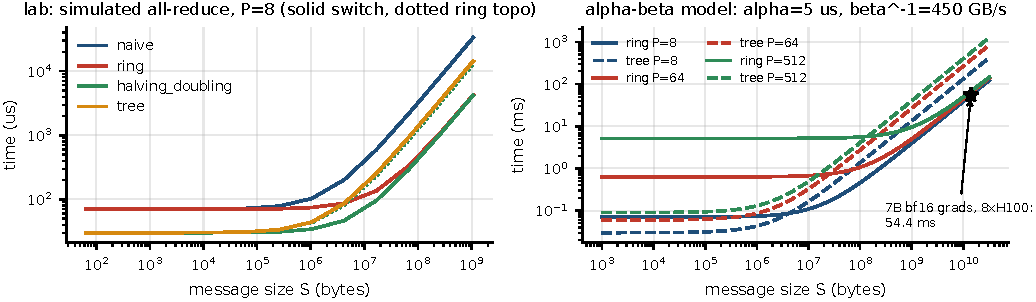
\includegraphics[width=\textwidth]{fig_allreduce}
\caption{all-reduce 时间随消息大小的变化。左：本文配套实验（15-849 分布式训练）的集合通信模拟器，$P=8$，$\alpha=5$~\textmu s，$1/\beta=450$~GB/s；
实线为交换机（全互联）拓扑，虚线为物理环拓扑。所有算法真实搬运 numpy 数组并逐 rank 计字节，模拟时间与闭式公式一致到 $10^{-12}$。
右：闭式 $\alpha$--$\beta$ 模型下 ring 与二项树在 $P=8,64,512$ 时的对比；五角星为 7B 模型 BF16 梯度（14~GB）在 8 卡 NVLink 上的 ring all-reduce（54.4~ms）。
小消息由延迟项主导（树赢），大消息由带宽项主导（ring 赢），交叉点随 $\alpha/\beta$ 与 $P$ 移动。}
\label{fig:allreduce}
\end{figure*}

图~\ref{fig:allreduce} 是这些公式的可视化。\lab{15-849 分布式训练}的模拟器在 $P=8$ 时给出：1~KB 消息 ring 70~\textmu s、树 30~\textmu s；
ring 在约 4.27~MB 处反超树；1~GB 时 ring 4.25~ms、树 14.3~ms；递归减半--倍增在交换机拓扑上与 ring 相当（4.21~ms），但在物理环上因链路争用慢到 12.56~ms，约 3 倍。
$P=64$、1~KB 时 ring 630~\textmu s 而树只有 60~\textmu s——这就是 NCCL 在大规模集群上引入 tree/双二叉树算法的原因。
唯一的真实测量是 CPU 上的 gloo：world=2 时 1~KB 0.40~ms、16~MB 25.8~ms，拟合 $\alpha\approx181$~\textmu s、等效带宽约 0.97~GB/s，只说明数量级。

\begin{est}{7B 模型的梯度 all-reduce 要多久？}
BF16 梯度 $S=2\times7\times10^9=14$~GB。8 卡 H100 节点内 NVLink 单向 450~GB/s，由式~\eqref{eq:ring}，带宽项
$2\times\frac{7}{8}\times14\times10^9/450\times10^9\approx54$~ms（\texttt{mlsys\_calc.ring\_allreduce\_time}，54.4~ms）。
若跨节点走每卡 400~Gb/s（50~GB/s）的 InfiniBand，约 0.49~s。一个 7B 模型在 8 卡上的单步计算若为数百毫秒，
那么跨节点时通信必须与反向重叠（分桶）、或者用分层 all-reduce（节点内 reduce-scatter、节点间 all-reduce、节点内 all-gather）。
\end{est}

\begin{qa}{all-reduce 为什么可以拆成 reduce-scatter + all-gather？这有什么用？}
\ans 先把和按分片算好（每卡得到 $1/p$ 的完整和），再把分片广播给所有人，结果与直接 all-reduce 相同。拆开之后可以只做一半：
ZeRO-2 只需要 reduce-scatter（每卡只更新自己负责的那份参数），ZeRO-3/FSDP 在前向用 all-gather 收集权重，序列并行用 RS+AG 替代 all-reduce
并在中间把激活按序列切分。
\wrong 「all-reduce 是原子操作，不能拆」。
\end{qa}

\begin{qa}{ring 和 tree all-reduce 怎么选？「环越大越慢」对吗？}
\ans ring 的带宽项 $2(p-1)S\beta/p$ 最优且几乎与 $p$ 无关，但延迟项 $2(p-1)\alpha$ 随 $p$ 线性增长；树的延迟项是 $O(\log p)$，带宽项差 $\log p$ 倍。
小消息（延迟主导）用树，大消息（带宽主导）用 ring；NCCL 根据消息大小与拓扑自动选择，并对大消息做分块流水。
\wrong 「ring 总是最好」或「环越大越慢」——变慢的只是延迟项，带宽项不变。
\end{qa}

\subsection{ZeRO 与 FSDP}

混合精度 Adam 的静态显存为每参数 16 字节：BF16 权重 $2N$、BF16 梯度 $2N$、FP32 主权重 $4N$、Adam 一阶矩 $4N$ 与二阶矩 $4N$
（后三项合称优化器状态 $12N$）~\cite{rajbhandari2020zero}。数据并行让每张卡都存一份完整的 $16N$，是巨大的冗余。
ZeRO~\cite{rajbhandari2020zero} 分三级消除冗余（$d$ 为 DP 度）：
\begin{equation}
\begin{gathered}
M_{\text{ZeRO-1}} = 4N+\frac{12N}{d},\qquad
M_{\text{ZeRO-2}} = 2N+\frac{14N}{d},\\
M_{\text{ZeRO-3}} = \frac{16N}{d}.
\end{gathered}
\label{eq:zero}
\end{equation}
ZeRO-1 只切优化器状态，ZeRO-2 再切梯度（reduce-scatter 代替 all-reduce），ZeRO-3 再切权重（前向、反向各 all-gather 一次）。
通信量方面，DP 的 all-reduce 等价于 RS+AG，每卡约 $2\Psi$（$\Psi$ 为参数字节数）；ZeRO-1/2 相同；ZeRO-3 是前向 AG + 反向 AG + 梯度 RS，共 $3\Psi$，
即 DP 的 1.5 倍。PyTorch FSDP~\cite{zhao2023pytorch} 是 ZeRO-3 的工程化实现：以模块为单位（FSDP unit）分片与 all-gather，
预取下一个 unit 的参数以重叠通信，并支持节点内分片、节点间复制的混合分片（HSDP）以降低跨节点流量。

\begin{table}[!t]
\centering
\caption{训练静态显存（GB/卡，不含激活；\texttt{mlsys\_calc.training\_memory\_bytes}）}
\label{tab:trainmem}
\footnotesize
\begin{tabularx}{\columnwidth}{@{}l c Y Y Y Y@{}}
\toprule
模型 & DP & 不切 & ZeRO-1 & ZeRO-2 & ZeRO-3 \\
\midrule
7B（$N=7\times10^9$） & 8 & 112.0 & 38.5 & 26.3 & 14.0 \\
Llama-3-8B（8.03B） & 8 & 128.5 & 44.2 & 30.1 & 16.1 \\
Llama-3-8B & 64 & 128.5 & 33.6 & 17.8 & 2.0 \\
Llama-3-70B（70.6B） & 8 & 1128.9 & 388.1 & 264.6 & 141.1 \\
Llama-3-70B & 64 & 1128.9 & 295.4 & 156.5 & 17.6 \\
\bottomrule
\end{tabularx}
\end{table}

\begin{est}{Llama-3-8B 与 70B 的训练显存}
8B：$16N=16\times8.03\times10^9\approx128.5$~GB，单卡放不下；8 卡 ZeRO-1 为 $4N+12N/8=32.1+12.0=44.2$~GB，ZeRO-3 为 16.1~GB（表~\ref{tab:trainmem}）。
70B：$16N\approx1.13$~TB。即使 64 卡 ZeRO-2 仍需 156.5~GB/卡（因为每卡保留完整 BF16 权重 141~GB），只有 ZeRO-3 或 TP/PP 能把权重切开。
激活另算：按 Korthikanti 等人的估计~\cite{korthikanti2023reducing}，使用 FlashAttention 时每层约 $34sbh$ 字节（$s$ 序列长、$b$ micro-batch、$h$ 隐藏维），
70B（$h=8192$，80 层）一条 4096 序列约 91~GB，全量重计算后只保留每层输入 $2sbh$，约 5.4~GB。图~\ref{fig:trainmem} 给出完整分解。
\end{est}

\begin{figure*}[!t]
\centering
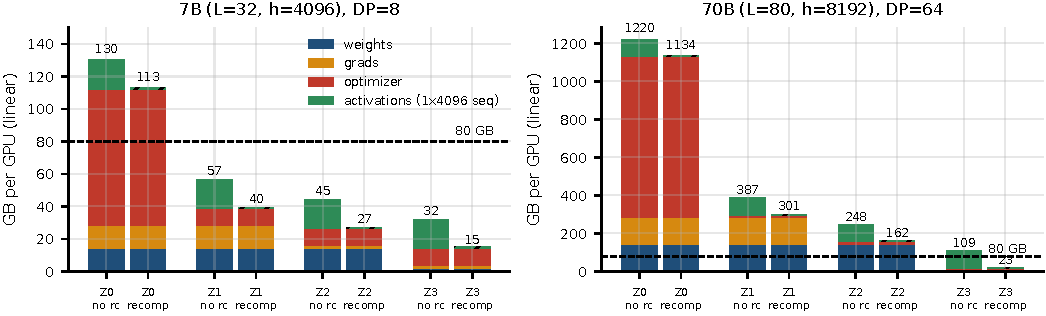
\includegraphics[width=\textwidth]{fig_train_memory}
\caption{每卡训练显存分解：权重、梯度、优化器状态与激活（micro-batch 为 1 条 4096 token 序列，按 Korthikanti 等人的 $34sbh$/层估计，
recomp 表示全量重计算只保留 $2sbh$/层）。左：7B（Llama-2 形状），DP=8；右：70B（Llama-3 形状），DP=64。虚线为 80~GB。
7B 在 ZeRO-1 + 重计算后即可放入单卡（40~GB）；70B 只有 ZeRO-3 才能放下，且激活在 ZeRO-3 下成为最大项（不重计算时 109~GB）。
激活公式针对 GPT 式 $4h$ MLP，对 SwiGLU 只是近似。}
\label{fig:trainmem}
\end{figure*}

\lab{15-849 分布式训练}在 4 个模拟 rank 上用显式的 reduce-scatter/all-gather 实现了 ZeRO 0--3（FP64、分片 Adam），20 步后参数与单进程训练最大差 $2.9\times10^{-16}$；
每 rank 常驻字节是 DP 的 1、0.625、0.4375、0.25（FP64 下 params:grads:m:v=1:1:1:1，理论比例为 $1$、$(2+2/P)/4$、$(1+3/P)/4$、$1/P$），
ZeRO-3 的通信恰好是 DP 的 1.5 倍。按论文的混合精度口径，$\Psi=7.5$B、$N_d=64$ 时计算器给出 120 / 31.4 / 16.6 / 1.88~GB，与 ZeRO 论文图 1 一致~\cite{rajbhandari2020zero}。

\begin{qa}{ZeRO 三个 stage 分别切了什么？通信量变不变？}
\ans stage 1 切优化器状态，stage 2 再切梯度，stage 3 再切权重。1、2 的通信量与 DP 相同（all-reduce=RS+AG，stage 2 只是把 AG 移到参数更新之后），
stage 3 在前向与反向各多一次权重 all-gather，是 DP 的 1.5 倍。7B、8 卡的静态显存依次为 112、38.5、26.3、14~GB。
\wrong 「ZeRO-3 的通信是 DP 的 3 倍」；或「ZeRO 改变了数学，会影响收敛」——它与 DP 数学等价。
\end{qa}

\subsection{张量并行（Megatron-LM）}

Megatron-LM~\cite{shoeybi2019megatron} 把 Transformer 的每一层沿隐藏维切分到 $t$ 张卡。MLP $Y=\mathrm{GeLU}(XW_1)W_2$ 中，$W_1$ 按列切，
每卡得到 $\mathrm{GeLU}$ 输入的一部分列；GeLU 是逐元素的，可本地计算；$W_2$ 按行切，正好消费这部分列，得到部分和，一次 all-reduce 求和。
attention 按头切分，$W_O$ 按行切，同样一次 all-reduce。用共轭算子 $f$（前向恒等、反向 all-reduce）与 $g$（前向 all-reduce、反向恒等）表示，
每层前向 2 次、反向 2 次 all-reduce，每次消息为 $b\cdot s\cdot h$ 个元素，与 $t$ 无关。

\begin{est}{张量并行每步要传多少？}
70B：$h=8192$，每卡一步处理 $b\cdot s=8192$ 个 token，BF16 下每次 all-reduce 的消息为 $8192\times8192\times2\approx134$~MB；每层 4 次、80 层约 43~GB/卡/步。
ring 因子 $2(t-1)/t=1.75$，走 450~GB/s NVLink 约 0.17~s，走 50~GB/s IB 约 1.5~s。这些通信在关键路径上，难以与计算重叠，
所以 TP 留在节点内。\lab{15-849 分布式训练}对 Llama-3-8B（batch 1、$s=8192$、$t=8$）的模型值为每次 67.1~MB、0.331~ms，32 层每步 42.4~ms；
TP 切分前后的前向、输入梯度与参数梯度最大差 $\le8.9\times10^{-16}$。
\end{est}

\begin{qa}{Megatron 的 MLP 为什么第一层按列切、第二层按行切？}
\ans 列切后每卡得到 $XW_1$ 的一部分列，GeLU 逐元素可本地算；行切的 $W_2$ 正好消费这部分列，输出部分和，一次 all-reduce 即可。
整个 MLP 前向只有一次通信。若两层都列切，第二层需要完整的输入，中间必须先 all-gather，通信更多。
\wrong 「两层都按列切更省通信」。
\end{qa}

\begin{qa}{为什么张量并行不出节点，而流水线并行可以跨节点？}
\ans TP 每层前反向共 4 次 $b\cdot s\cdot h$ 的 all-reduce，处在关键路径上、难以重叠，必须走 NVLink（450~GB/s）；PP 只在 stage 边界点对点传激活，
每个 micro-batch 一次 $b\cdot s\cdot h$，量小且可以与计算重叠，走 IB（50~GB/s，约为 NVLink 的 1/9）也可接受。
\wrong 「随便放」或「TP 通信量小所以可以跨节点」。
\end{qa}

\subsection{序列并行与上下文并行}

TP 并没有切分 LayerNorm 与 dropout 的激活，这部分在长序列下很可观。Korthikanti 等人的序列并行（SP）~\cite{korthikanti2023reducing}
在这些区域沿序列维切分，把 TP 的 all-reduce 换成 reduce-scatter + all-gather：通信量相同，激活却按 $t$ 切分。
当序列长到单卡放不下 attention 的输入时，需要上下文并行（CP）：Ring Attention~\cite{liu2023ring} 把序列切到 $c$ 张卡，
$K/V$ 块沿环传递，每卡用 online softmax（式~\eqref{eq:online}）累加，通信与块计算重叠；DeepSpeed-Ulysses~\cite{jacobs2023deepspeed}
则在 attention 前后各做一次 all-to-all，把「按序列切」转换为「按头切」，通信量与 $c$ 无关但并行度受头数限制。

\subsection{流水线并行}

流水线并行（PP）把层切成 $p$ 个 stage，一个 mini-batch 切成 $m$ 个 micro-batch。GPipe~\cite{huang2019gpipe} 先做完全部前向再做全部反向，
PipeDream~\cite{narayanan2019pipedream} 的 1F1B 调度在稳态中交替一个前向与一个反向。填充与排空各需 $p-1$ 个时隙，故两者的气泡比例相同：
\begin{equation}
\text{bubble} = \frac{p-1}{m+p-1},\qquad
\text{bubble}_{\text{interleaved}} = \frac{(p-1)/v}{m+(p-1)/v},
\label{eq:bubble}
\end{equation}
其中交错调度（interleaved 1F1B）让每卡负责 $v$ 个不相邻的虚拟 stage~\cite{narayanan2021efficient}，气泡缩小 $v$ 倍，代价是 $v$ 倍的点对点通信。
1F1B 的真正收益是\emph{激活显存}：在途的 micro-batch 从 $m$ 降到最多 $p$。

\begin{figure*}[!t]
\centering
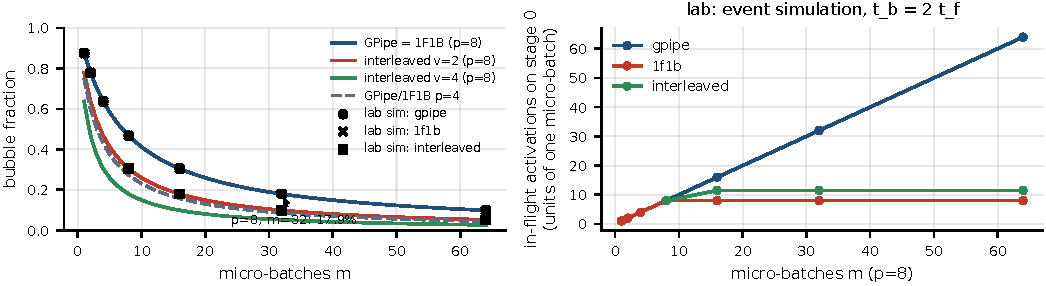
\includegraphics[width=\textwidth]{fig_pipeline}
\caption{流水线气泡与在途激活。左：式~\eqref{eq:bubble} 的气泡比例随 micro-batch 数 $m$ 的变化（$p=8$，$v=1,2,4$；虚线 $p=4$），
黑色标记为配套实验离散事件模拟的结果（$t_b=2t_f$），与公式一致到 $10^{-12}$。$p=8,m=32$ 时气泡为 17.9\%。
右：0 号 stage 的峰值在途激活。GPipe 随 $m$ 线性增长；1F1B 封顶于 $p=8$；交错调度（$v=2$）气泡减半，但在途激活升到 11.5 份，多于 1F1B。}
\label{fig:pipeline}
\end{figure*}

\begin{est}{8 级流水线、32 个 micro-batch 的气泡}
$p=8$、$m=32$：$7/39\approx17.9\%$；$m=8$ 时为 46.7\%，所以经验上取 $m\ge4p$。交错 $v=2$ 时为 9.9\%，$v=4$ 时为 5.2\%
（\texttt{mlsys\_calc.pipeline\_bubble}）。配套模拟中 $p=4,m=8$ 的 GPipe 与 1F1B 气泡都是 0.273，交错 $v=2$ 为 0.158；
但 0 号卡的在途激活 GPipe/1F1B/交错分别为 8/4/5.5 份——气泡与激活显存之间存在真实的权衡（图~\ref{fig:pipeline}）。
\end{est}

\begin{qa}{1F1B 比 GPipe 好在哪？它减少了气泡吗？}
\ans 均匀 stage 下两者的气泡完全相同，都是 $(p-1)/(m+p-1)$。1F1B 在稳态每做一个前向就做一个反向，一个 micro-batch 的反向做完就释放它的激活，
在途激活从 $m$ 份降到 $p$ 份，因此可以用更大的 $m$ 来\emph{间接}降低气泡。真正减小气泡的是交错调度（除以 $v$），代价是 $v$ 倍的点对点通信与更多在途激活。
\wrong 「1F1B 的气泡比 GPipe 小」。
\end{qa}

\subsection{3D 并行的规划}

表~\ref{tab:parallel} 比较了各类并行策略切分的对象、通信模式与适用范围。Narayanan 等人~\cite{narayanan2021efficient} 总结的规划经验可以写成一个可复述的流程：
（1）TP 度 $t$ 取节点内 GPU 数（通常 8），因为 TP 通信量最大且在关键路径上；（2）PP 度 $p$ 取能放下模型的最小值，因为 stage 越多气泡越大；
（3）剩余维度给 DP，并配 ZeRO-1 与梯度分桶重叠；（4）$m\ge4p$ 以控制气泡，同时检查 global batch 不超过收敛允许的临界 batch；
（5）长序列再加 SP/CP，MoE 再加专家并行（第~\ref{sec:eff} 节）。Alpa~\cite{zheng2022alpa} 把算子内（TP/DP）与算子间（PP）并行分层求解，
GSPMD~\cite{xu2021gspmd} 通过 sharding 注解让编译器自动插入通信，它们是「自动并行」的代表。

\begin{table*}[!t]
\centering
\caption{并行策略对比（$N$ 参数量，$s$ 每元素字节，$b\cdot s_{\text{seq}}\cdot h$ 为一个 micro-batch 的激活张量）}
\label{tab:parallel}
\footnotesize
\begin{tabularx}{\textwidth}{@{}l L{2.4cm} L{3.4cm} L{3.6cm} Y@{}}
\toprule
策略 & 切分对象 & 每步通信 & 显存收益 & 适用与代价 \\
\midrule
DP~\cite{li2020pytorch} & 数据 & 梯度 all-reduce，$\approx2Ns$/卡 & 无（每卡完整 $16N$） & 最简单；受 global batch 与显存限制 \\
ZeRO-1/2~\cite{rajbhandari2020zero} & 优化器状态/梯度 & 同 DP（RS+AG） & $4N+12N/d$ / $2N+14N/d$ & 几乎免费的显存收益，默认开启 \\
ZeRO-3 / FSDP~\cite{rajbhandari2020zero,zhao2023pytorch} & 参数、梯度、状态 & $1.5\times$ DP（AG+AG+RS） & $16N/d$ & 模型放不下且不愿改模型代码；跨 IB 时通信重 \\
TP~\cite{shoeybi2019megatron} & 层内权重（隐藏维/头） & 每层 4 次 $bs_{\text{seq}}h$ all-reduce & 权重、梯度、部分激活 $/t$ & 节点内（NVLink）；$t$ 受头数与效率限制 \\
SP~\cite{korthikanti2023reducing} & LayerNorm/dropout 激活（序列维） & 与 TP 相同（RS+AG 替代 AR） & 剩余激活 $/t$ & 与 TP 配合，几乎无额外代价 \\
CP~\cite{liu2023ring,jacobs2023deepspeed} & 序列（attention） & ring 传 K/V 或 2 次 all-to-all & 激活与 attention 输入 $/c$ & 长上下文训练/prefill \\
PP~\cite{huang2019gpipe,narayanan2019pipedream} & 层（stage） & stage 边界点对点 $bs_{\text{seq}}h$ & 权重与状态 $/p$ & 可跨节点；气泡 $(p-1)/(m+p-1)$ \\
EP~\cite{lepikhin2021gshard,fedus2022switch} & MoE 专家 & 每层 2 次 all-to-all（前向） & 专家参数 $/e$ & MoE；负载均衡与 all-to-all 带宽 \\
\bottomrule
\end{tabularx}
\end{table*}

\begin{est}{70B 模型预训练 15T token 需要多少卡、多少天？}
$C=6ND=6\times70.6\times10^9\times15\times10^{12}\approx6.35\times10^{24}$~FLOP。H100、MFU 40\%：1024 卡需
$6.35\times10^{24}/(1024\times989\times10^{12}\times0.4)\approx1.57\times10^7$~s $\approx181$ 天；8192 卡约 23 天（图~\ref{fig:chinchilla} 右）。
显存：TP=8（节点内）$\times$ PP=4 时每卡静态显存 $16N/32\approx35$~GB；再加 DP=256 的 ZeRO-1 为 $4N/32+12N/(32\times256)\approx8.9$~GB，留出空间给激活。
DP 梯度每卡分片 $2N/32\approx4.4$~GB，在 IB 上 ring all-reduce 约 $2\times4.4/50\approx0.18$~s，可藏在反向里。
\end{est}

\begin{qa}{70B 训练为什么不直接用 FSDP/ZeRO-3，而用 TP+PP+DP？}
\ans 两种都可行，取舍在通信位置。ZeRO-3 每层前向、反向都要 all-gather 权重，跨 IB 的总通信是 DP 的 1.5 倍；TP+PP 把每层的大通信留在 NVLink 内，
跨节点只有 PP 的点对点和 DP 的梯度分片。规模越大、网络越慢，TP+PP 越有优势；而 FSDP 的优点是不改模型代码、调度简单，中等规模（数百卡）常常足够。
\wrong 「ZeRO-3 显存最省所以总是最好」。
\end{qa}

\subsection{激活重计算}

Chen 等人~\cite{chen2016training} 提出每 $k$ 层存一个检查点：显存约 $n/k+k$，取 $k=\sqrt{n}$ 时最小约 $2\sqrt{n}$，额外计算约一次前向
（总 FLOPs 从 $3F$ 变为 $4F$，即 $+33\%$）。Checkmate~\cite{jain2020checkmate} 把重计算建模为混合整数线性规划，在显存预算下求最优的保存/重算方案；
Korthikanti 等人~\cite{korthikanti2023reducing} 提出选择性重计算：只重算 attention 中占显存大但计算便宜的部分（softmax、dropout mask），开销仅几个百分点。
\lab{15-849 分布式训练}实现了链上的 $\sqrt{n}$ 与预算约束动态规划：均匀 64 层时 $\sqrt{n}$（每 8 层）峰值 15、重算 56，已在 Pareto 前沿上；
异构 32 层（大小与代价 $\in[1,8]$）在同为 53 的预算下，$\sqrt{n}$ 重算 117 而 DP 只需 85，少 27\%（图~\ref{fig:labkvsys} 右）。
torch 版 16 层实验中 4 层一段（$=\sqrt{16}$）峰值最低，梯度与不重计算逐位相等；CPU 上时间开销 1.52 倍，远高于理论 1.33 倍，是 Python 钩子开销，不能外推到 GPU。

\begin{qa}{激活重计算多花多少算力？}
\ans 全量重计算多一次前向，前向:反向 $=1:2$，总计算从 $3F$ 到 $4F$，即 $+33\%$，不是翻倍。按 $\sqrt{n}$ 设检查点时激活从 $O(n)$ 降到 $O(\sqrt{n})$。
选择性重计算只重算 softmax/dropout 等，开销通常 $<5\%$。报告 MFU 时不计重算 FLOPs，HFU 计入。
\wrong 「重计算让训练慢一倍」。
\end{qa}

\subsection{混合精度、offload 与 FP8}

Micikevicius 等人~\cite{micikevicius2018mixed} 的混合精度训练确立了三件事：FP16 计算、FP32 主权重、动态 loss scaling。
BF16~\cite{kalamkar2019study} 有 8 位指数，与 FP32 动态范围相同，通常不需要 loss scaling，但只有 7 位尾数；
无论哪种，求和、softmax、LayerNorm 统计量与 loss 都应在 FP32 中累加。

ZeRO-Offload~\cite{ren2021zero} 把优化器状态与 Adam 更新放到 CPU，只在 GPU 上做前反向；ZeRO-Infinity~\cite{rajbhandari2021zero} 进一步利用 NVMe。
它们的瓶颈是 PCIe：7B 模型每步向主机传 $2N=14$~GB 梯度、再传回 14~GB 权重，在 32~GB/s 的 PCIe 4.0 上各约 0.44~s，所以 offload
只在单步计算足够长（大 batch）时才划算。

FP8 有 E4M3（精度更高，用于前向权重与激活）与 E5M2（范围更大，用于梯度）两种格式~\cite{micikevicius2022fp8}，H100 上算力是 BF16 的 2 倍。
由于动态范围窄，需要按张量（或更细粒度）缩放，常用 delayed scaling：用前若干步的 amax 历史估计当前 scale。DeepSeek-V3 报告了用细粒度（分块）缩放的
FP8 训练~\cite{deepseekai2024v3}。风险主要在离群值与累加精度，主权重与优化器状态仍为高精度。

\begin{qa}{BF16 和 FP16 训练的区别？FP8 训练要注意什么？}
\ans BF16 有 8 位指数、7 位尾数，范围同 FP32，不需要 loss scaling；FP16 有 5 位指数、10 位尾数，精度更高但梯度容易下溢，必须动态 loss scaling。
两者都要 FP32 主权重与 FP32 累加。FP8 需要 per-tensor/per-block 的 scale（delayed scaling 用 amax 历史），前向用 E4M3、梯度用 E5M2；
注意激活离群值、GEMM 累加精度，以及哪些算子（LayerNorm、softmax、loss）必须留在高精度。
\wrong 「BF16 精度比 FP16 高」；「FP8 训练就是把所有张量转成 8 位」。
\end{qa}

\begin{keypts}
\begin{itemize}
\item ring all-reduce：$2(p-1)\alpha+2(p-1)S\beta/p$；小消息用树、大消息用 ring；7B 梯度 8 卡 NVLink 约 54~ms。
\item $16N$：7B 单卡 112~GB；ZeRO-1/2/3 公式见式~\eqref{eq:zero}；ZeRO-3 通信 1.5 倍。
\item Megatron：列切 + 行切，每层前反向 4 次 $bsh$ all-reduce，留在节点内。
\item 气泡 $(p-1)/(m+p-1)$；1F1B 省激活不省气泡；交错除以 $v$。
\item 重计算 $+33\%$ FLOPs；选择性重计算 $<5\%$；BF16 免 loss scaling；FP8 需要 scale 管理。
\end{itemize}
\end{keypts}

\begin{research}
\begin{itemize}
\item 3D 并行的自动规划（Alpa、GSPMD）通常以静态代价模型为基础，而真实集群的带宽随拓扑与拥塞变化。可做的实验：
在 $\alpha$--$\beta$ 模型中加入拓扑项（交换机 vs 物理环，本文实验显示 halving-doubling 在物理环上慢 3 倍），看最优并行配置是否改变。
\item 流水线调度的「零气泡」方向~\cite{qi2024zerobubble}（把反向拆成对输入与对权重两部分分别调度）与激活显存的关系值得系统测量：
在本文的事件模拟器中把 $t_b$ 拆为 $t_{b,x}+t_{b,w}$，比较气泡与峰值激活的 Pareto 前沿。
\end{itemize}
\end{research}
